\chapter{Network Searching}

\section{Hubs and Authorities}

\begin{itemize}
    \item Used to identify important nodes in a network
    \item Hubs are nodes that point to many authorities
    \item Authorities are nodes that are pointed to by many hubs
\end{itemize}

\subsection{Measuring Rankings}

\begin{itemize}
    \item Authority score: sum of scores of hubs pointing to the authority
    \item Hub score: sum of scores of authorities pointed to by the hub
    \item HITS: iteratively update authority and hub scores
\end{itemize}

\subsection{Example Using Adjacency Matrix}

\begin{figure}[!htbp]
    \centering
    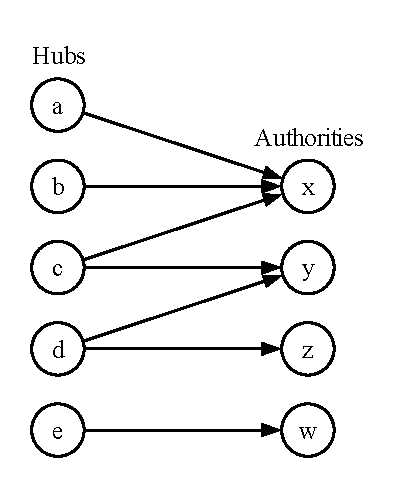
\includegraphics[height=5cm]{figures/hits-bipartite.pdf}
    \caption{Bipartite network of hubs pointing to authorities.}
\end{figure}

\begin{itemize}
    \item Node order: hubs \((a,b,c,d,e)\); authorities \((x,y,z,w)\)
    \item Adjacency matrix \(A\): rows = hubs; columns = authorities
\end{itemize}

\[
    A =
    \begin{bmatrix}
        1 & 0 & 0 & 0 \\
        1 & 0 & 0 & 0 \\
        1 & 1 & 0 & 0 \\
        0 & 1 & 1 & 0 \\
        0 & 0 & 0 & 1
    \end{bmatrix}
\]

\begin{itemize}
    \item Initialize hub scores: \(\mathbf{h}^{(0)}=(1,1,1,1,1)\)
    \item Each iteration: \(\mathbf{a}^{(t)}=A^\mathsf{T}\mathbf{h}^{(t-1)}\); \(\mathbf{h}^{(t)}=A\mathbf{a}^{(t)}\)
    \item Integer updates below: no intermediate normalization; reported scores normalized to unit \(L_2\) length
\end{itemize}

\begin{itemize}
    \item Iteration 1:
          \[
              \begin{aligned}
                  \mathbf{a}^{(1)} & = A^\mathsf{T}\mathbf{h}^{(0)}=(3,2,1,1),
                                   & \widehat{\mathbf{a}}^{(1)}                & \approx(0.775,0.516,0.258,0.258)       \\
                  \mathbf{h}^{(1)} & = A\mathbf{a}^{(1)}=(3,3,5,3,1),
                                   & \widehat{\mathbf{h}}^{(1)}                & \approx(0.412,0.412,0.687,0.412,0.137)
              \end{aligned}
          \]

    \item Iteration 2:
          \[
              \begin{aligned}
                  \mathbf{a}^{(2)} & = A^\mathsf{T}\mathbf{h}^{(1)}=(11,8,3,1),
                                   & \widehat{\mathbf{a}}^{(2)}                 & \approx(0.788,0.573,0.215,0.072)       \\
                  \mathbf{h}^{(2)} & = A\mathbf{a}^{(2)}=(11,11,19,11,1),
                                   & \widehat{\mathbf{h}}^{(2)}                 & \approx(0.409,0.409,0.706,0.409,0.037)
              \end{aligned}
          \]

    \item Iteration 3:
          \[
              \begin{aligned}
                  \mathbf{a}^{(3)} & = A^\mathsf{T}\mathbf{h}^{(2)}=(41,30,11,1),
                                   & \widehat{\mathbf{a}}^{(3)}                   & \approx(0.789,0.577,0.212,0.019)       \\
                  \mathbf{h}^{(3)} & = A\mathbf{a}^{(3)}=(41,41,71,41,1),
                                   & \widehat{\mathbf{h}}^{(3)}                   & \approx(0.408,0.408,0.707,0.408,0.010)
              \end{aligned}
          \]
\end{itemize}

\begin{itemize}
    \item Iteration 3 ranking: \(c\) strongest hub; \(x\) strongest authority
    \item Ranking trend: \(c\) and \(x\) dominant; \(e\) and \(w\) increasingly weak
\end{itemize}

\section{PageRank}

\begin{itemize}
    \item Method for ranking nodes in a network based on the structure of incoming links
    \item Counts the number and quality of links to a page to determine its importance
          \begin{enumerate}
              \item Assign equal scores to all nodes: $\frac{1}{n}$
              \item Update scores based on the scores of incoming links, typically using the formula: \(\PR(i) = \sum_{j \in M(i)} \frac{\PR(j)}{L(j)}\) where $M(i)$ is the set of nodes linking to $i$ and $L(j)$ is the number of outbound links from node $j$
          \end{enumerate}
\end{itemize}